% Provenance (never printed): old terminale S material on the continental crust
% (granitic composition, thickness, density, age; roots and isostasy). Thickness
% from Christensen-Mooney 1995 and Cogley 1984 (CRUST1.0 dropped: no licence,
% Sync 1); ocean-floor ages from figdata/grade-12/crust_ages.py (Seton 2020 grid,
% as in g11.01). Airy isostasy is g11.03's: recalled, not re-derived. Radiometric
% dating is g12.07's: ages are only quoted here.
\chapter{De continentale korst}\label{ch:g12:continental-crust}

In het noordwesten van Canada, bij de Acasta-rivier, dagzoomt een grijs gesteente
met lichte en donkere banden. Het is gedateerd op 4.00 tot 4.03 miljard
jaar: de gneis van Acasta, het oudste bekende gesteente. Nog ouder zijn korrels van
het mineraal zirkoon, elk een fractie van een millimeter lang, gevonden in oude
sedimentaire gesteenten van de Jack Hills in West-Australië. Afgesleten van oudere
gesteenten en door water meegevoerd voordat ze werden begraven, kristalliseerden ze 4.4
miljard jaar geleden, en ze tonen dat er toen al een korst bestond. Geen enkele oceaanbodem is ook maar een twintigste zo oud. Dit hoofdstuk
vraagt waaruit de continenten bestaan, en waarom ze blijven bestaan.
% ledger: bowring99:acasta, wilde01:zircon, uw14:jack-hills, photo:g12-acasta, photo:g12-jack-hills-zircons

\begin{omfigure}
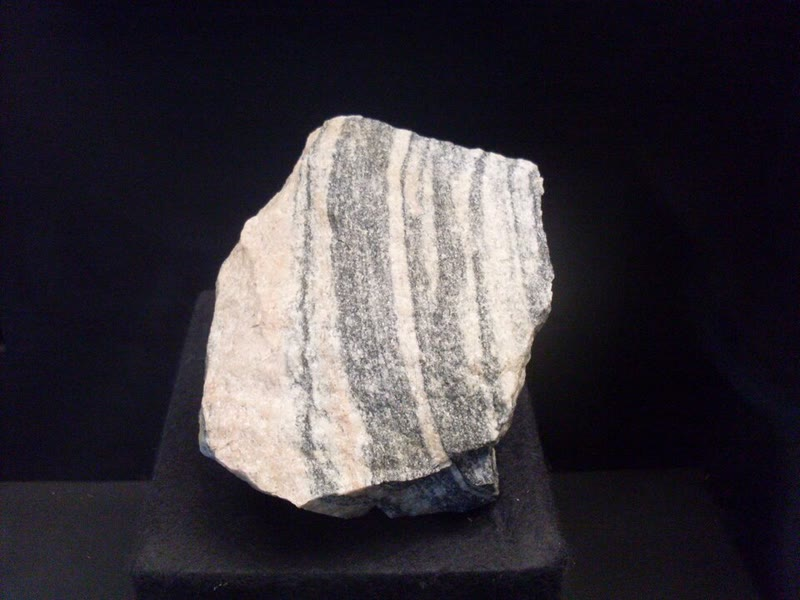
\includegraphics[height=4.6cm]{images/book2/g12-pedro-acasta-gneiss.jpg}\hspace{0.04\linewidth}%
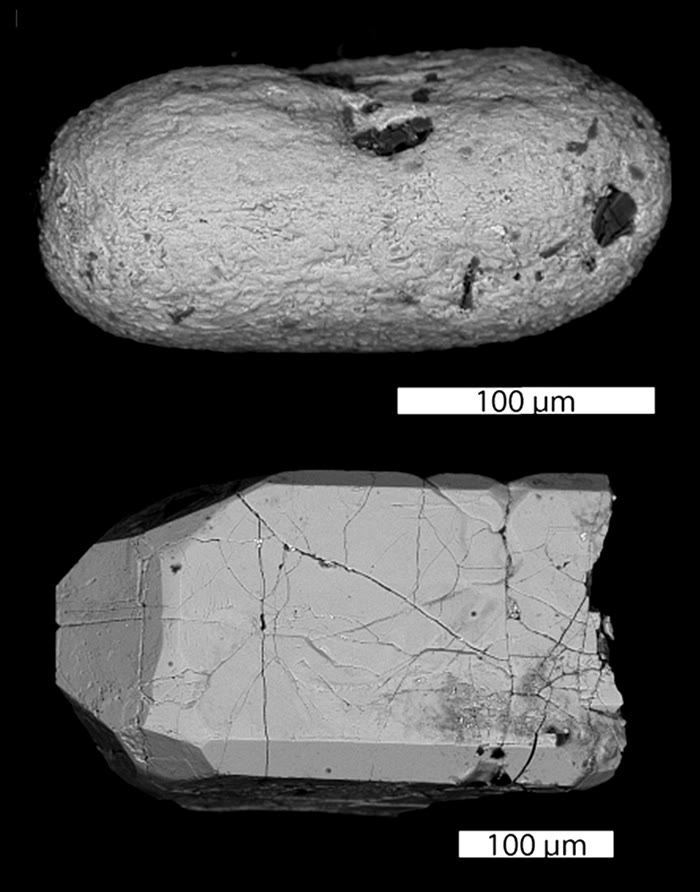
\includegraphics[height=4.6cm]{images/book2/g12-cavosie-jack-hills-zircons.jpg}

{\small Links: een stuk van de gneis van Acasta, 4.03 miljard jaar oud, in een
museumvitrine. Foto Pedroalexandrade (CC~BY-SA~3.0). Rechts: twee
zirkoonkorrels uit de Jack Hills, West-Australië, gezien met een
elektronenmicroscoop; elke schaalstreep is \qty{100}{\micro m}. De bovenste korrel werd
afgerond toen hij door water werd meegevoerd, de onderste behield zijn kristalvlakken.
Beelden A.~Cavosie en J.~Valley (publiek domein).}
\end{omfigure}
% ledger: photo:g12-acasta, photo:g12-jack-hills-zircons

\begin{recall}
De korst eindigt bij de \omterm{def:g11:seismic-structure:moho}{Moho}, waaronder de dichtere mantel ligt
(\cref{ch:g11:seismic-structure}). De \omterm{def:g11:ocean-ridges:oceanic-lithosphere}{oceanische korst} is ongeveer \qty{7}{km}
basalt en \omterm{def:g11:ocean-ridges:gabbro}{gabbro}, gemaakt bij de ruggen (\cref{ch:g11:ocean-ridges}), en ze is
nooit ouder dan ongeveer 190 miljoen jaar (\cref{ch:g11:drift-to-spreading}).
De buitenste lagen drijven op de \omterm{def:g11:lithosphere-asthenosphere:lithosphere}{asthenosfeer}: in het model van Airy heeft een gebied dat
een hoogte $h$ hoger staat, een korst die dikker is met $h\,\rho_m/(\rho_m -
\rho_c)$ (\cref{ch:g11:lithosphere-asthenosphere}). Stollingsgesteenten worden benoemd
naar hun \omterm{def:g11:igneous-rocks:texture}{textuur} en hun silicagehalte: \omterm{def:g11:igneous-rocks:felsic-mafic}{mafisch} van 45 tot
\qty{55}{\percent} \ce{SiO2}, \omterm{def:g11:igneous-rocks:felsic-mafic}{intermediair} van 55 tot 65, \omterm{def:g11:igneous-rocks:felsic-mafic}{felsisch} van 65 tot
75 (\cref{ch:g11:igneous-rocks}). Radioactieve elementen vervallen in een constant
tempo, en dat geeft gesteenten hun ouderdom (de natuurkundeboeken;
\cref{ch:g12:age-of-the-earth}).
\end{recall}
% ledger: white92:crust, data:b2-seafloor-age, tulane:magma-types

\section{Waaruit de continenten bestaan}

\begin{definition}[Continentale korst]\label{def:g12:continental-crust:continental-crust}
De \emph{continentale korst}\index{continentale korst} is de korst die
de continenten vormt, ook de delen ervan onder ondiepe zeeën. Ze is
dik, in haar bovenste deel gemiddeld granitisch van samenstelling, licht, en ze
kan heel oud zijn.
\end{definition}
% ledger: tulane:crust-types, tulane:roots, cogley84:continents

De continenten zijn groter dan het land. De randen van de \omterm{def:g12:continental-crust:continental-crust}{continentale korst}
liggen onder zee, op de continentale platten: zo in kaart gebracht beslaat de
\omterm{def:g12:continental-crust:continental-crust}{continentale korst} \num{210}~miljoen~\unit{km^2}, \qty{41}{\percent} van het
aardoppervlak, waarvan bijna een derde, \qty{30.6}{\percent},
onder water ligt. Met haar ondergelopen delen meegeteld ligt de gemiddelde hoogte van de
\omterm{def:g12:continental-crust:continental-crust}{continentale korst} maar ongeveer \qty{120}{m} boven zeeniveau.
% ledger: cogley84:continents

Aan het oppervlak tonen de continenten elke soort gesteente --- sedimenten,
vulkanische gesteenten, metamorfe gesteenten --- maar onder de sedimentaire bedekking bestaat de
\omterm{def:g12:continental-crust:continental-crust}{continentale korst} vooral uit granitische gesteenten en uit de metamorfe
en plutonische gesteenten van oude bergwortels. Gemiddeld bevat de hele \omterm{def:g12:continental-crust:continental-crust}{continentale
korst} \qty{60.6}{\percent} silica; haar bovenste deel is rijker,
\qty{66.6}{\percent}, dus haar diepere deel moet armer zijn.
% ledger: rg14:crust, tulane:crust-types, cm95:crust

\begin{omfigure}
\begin{tikzpicture}
\begin{axis}[omrecord, ybar=0pt, width=0.92\linewidth, height=5.0cm, bar width=7pt,
  ymin=0, ymax=80, ylabel={massafractie (\unit{\percent})},
  symbolic x coords={SiO2, Al2O3, FeO, MgO, CaO, Na2O, K2O},
  xticklabels={\ce{SiO2}, \ce{Al2O3}, \ce{FeO}, \ce{MgO}, \ce{CaO}, \ce{Na2O}, \ce{K2O}},
  xtick=data, enlarge x limits=0.08, ymajorgrids=true, xmajorgrids=false,
  legend style={font=\scriptsize, at={(0.98,0.97)}, anchor=north east, legend columns=1}]
% ledger: rg14:crust (upper and bulk continental crust; FeO* total iron)
\addplot[fill=omLithGranite, draw=black!60] coordinates {(SiO2,66.6) (Al2O3,15.4) (FeO,5.04) (MgO,2.48) (CaO,3.59) (Na2O,3.27) (K2O,2.80)};
\addplot[fill=omProp!55, draw=black!60] coordinates {(SiO2,60.6) (Al2O3,15.9) (FeO,6.71) (MgO,4.66) (CaO,6.41) (Na2O,3.07) (K2O,1.81)};
% ledger: earle:magma-oxides (mafic magma: midpoint of each range, the bar spans the range)
\addplot[fill=omLithBasalt, draw=black!60, error bars/.cd, y dir=both, y explicit]
  coordinates {(SiO2,50) +- (0,5) (Al2O3,16) +- (0,2) (FeO,10) +- (0,2) (MgO,7) +- (0,2) (CaO,9) +- (0,2) (Na2O,2) +- (0,1) (K2O,1.75) +- (0,1.25)};
\legend{bovenste continentale korst, hele continentale korst, mafisch magma (bereik)}
\end{axis}
\end{tikzpicture}

{\small Samenstelling van de \omterm{def:g12:continental-crust:continental-crust}{continentale korst} vergeleken met een \omterm{def:g11:igneous-rocks:felsic-mafic}{mafisch} magma, het
soort dat de \omterm{def:g11:ocean-ridges:oceanic-lithosphere}{oceanische korst} maakt: de belangrijkste oxiden, in procent van de massa
(\ce{FeO} telt al het ijzer). De \omterm{def:g12:continental-crust:continental-crust}{continentale korst} is rijker aan silica,
natrium en kalium, armer aan ijzer, magnesium en calcium. Gegevens: Rudnick
en Gao (2014); \omterm{def:g11:igneous-rocks:felsic-mafic}{mafisch} bereik uit S.~Earle, \emph{Physical Geology}
(CC~BY~4.0).}
\end{omfigure}
% ledger: rg14:crust, earle:magma-oxides

\section{Een dikke, lichte korst}

Seismisch onderzoek vindt de \omterm{def:g11:seismic-structure:moho}{Moho} onder de continenten op heel verschillende
diepten. Gemiddeld over alle continenten, gewogen naar oppervlakte, is de korst ongeveer
\qty{41}{km} dik; ze is dunner, ongeveer \qty{30}{km}, waar de korst is
uitgerekt, en dikker, gemiddeld ongeveer \qty{46}{km}, in gebergtegordels.
Buiten gebergtegordels is ze gewoonlijk 35 tot \qty{40}{km} dik; onder de
hoogste ketens 50 tot \qty{70}{km}, ongeveer \qty{70}{km} onder delen van Tibet.
De \omterm{def:g11:ocean-ridges:oceanic-lithosphere}{oceanische korst} is ongeveer \qty{7}{km} dik: de \omterm{def:g12:continental-crust:continental-crust}{continentale korst} is vijf
tot tien keer dikker.
% ledger: cm95:crust, tulane:roots, karplus:tibet-moho, white92:crust

\begin{omfigure}
\begin{tikzpicture}
\begin{axis}[omrecord, xbar, bar shift=0pt, width=0.78\linewidth, height=5.0cm, bar width=8pt,
  xmin=0, xmax=80, ymin=0.4, ymax=5.6, ytick={1,...,5},
  yticklabels={oceanische korst, uitgerekte continenten, continenten (gemiddeld), gebergtegordels (gemiddeld), onder Tibet},
  xlabel={dikte van de korst (\unit{km})}, ymajorgrids=false,
  nodes near coords, nodes near coords style={font=\scriptsize, anchor=west}, point meta=explicit symbolic]
% ledger: white92:crust, cm95:crust, karplus:tibet-moho
\addplot[fill=omLithBasalt, draw=black!60] coordinates {(7.1,1) [7.1]};
\addplot[fill=omLithGranite, draw=black!60] coordinates {(30.5,2) [30.5] (41.1,3) [41.1] (46.3,4) [46.3] (70,5) [ongeveer 70]};
\end{axis}
\end{tikzpicture}

{\small Dikte van de korst uit seismische metingen. Gegevens: White,
McKenzie en O'Nions (1992) voor de \omterm{def:g11:ocean-ridges:oceanic-lithosphere}{oceanische korst}; Christensen en Mooney
(1995) voor de continentale gemiddelden; Karplus en anderen (2019) voor Tibet.}
\end{omfigure}
% ledger: white92:crust, cm95:crust, karplus:tibet-moho

De \omterm{def:g12:continental-crust:continental-crust}{continentale korst} is ook licht. Haar gemiddelde dichtheid is ongeveer
\qty{2830}{kg/m^3}. Het basalt en \omterm{def:g11:ocean-ridges:gabbro}{gabbro} van de \omterm{def:g11:ocean-ridges:oceanic-lithosphere}{oceanische korst}, rijk aan
pyroxeen en olivijn, komen op ongeveer \qty{3000}{kg/m^3}
(\cref{ch:g11:minerals}), en de mantel net onder de \omterm{def:g11:seismic-structure:moho}{Moho} op ongeveer
\qty{3380}{kg/m^3}. Een dikke en lichte korst drijft hoog: daarom
staan de continenten boven de oceaanbodem, en daarom kan een continent niet
omlaag worden getrokken bij een \omterm{def:g11:subduction-zones:subduction}{subductiezone}. Waar een continent bij een trog aankomt, is het te
licht om te zinken; de \omterm{def:g11:subduction-zones:subduction}{subductie} stopt, en de twee continenten botsen
(\cref{ch:g12:mountain-building}). \omterm{def:g12:continental-crust:continental-crust}{Continentale korst} die eenmaal is gemaakt, is moeilijk te
vernietigen.
% ledger: cm95:crust, data:prem, tulane:roots, tulane:no-subduct
% values (mineral_density.py): basalt/gabbro rock line 3.0015 g/cm3

\begin{omfigure}
\begin{tikzpicture}[x=1cm, y=0.075cm, font=\footnotesize]
  % continental column: 41 km of crust, surface at +0.12 km (mean height); ocean column: 3.7 km of water drawn schematically
  \fill[omLithGranite] (0,0) rectangle (3,-41);
  \fill[omLithPeridotite!60] (0,-41) rectangle (3,-60);
  \fill[omSea] (6,0) rectangle (9,-4);
  \fill[omLithGabbro] (6,-4) rectangle (9,-11.1);
  \fill[omLithPeridotite!60] (6,-11.1) rectangle (9,-60);
  \draw[black!60] (0,0) rectangle (3,-60) (6,0) rectangle (9,-60);
  \draw[line width=0.9pt] (0,-41) -- (3,-41) (6,-11.1) -- (9,-11.1);
  \node[align=center] at (1.5,-20) {continentale korst\\ongeveer \qty{41}{km}\\\qty{2830}{kg/m^3}\\tot 4 miljard jaar};
  \node[align=center] at (7.5,-24) {mantel\\\qty{3380}{kg/m^3}\\onder de Moho};
  \node[align=center] at (1.5,-50.5) {mantel};
  \node at (7.5,-2) {oceaan};
  \draw[black!60] (8.6,-7.6) -- (9.3,-7.6);
  \node[anchor=west, align=left] at (9.3,-7.6) {oceanische korst,\\ongeveer \qty{7}{km}\\\qty{3000}{kg/m^3}\\minder dan 200 miljoen jaar};
  \node[anchor=east] at (-0.1,-41) {Moho};
  \node[anchor=east] at (5.9,-11.1) {Moho};
  \node[anchor=south] at (1.5,0) {een continent};
  \node[anchor=south] at (7.5,0) {een oceaan};
  \foreach \d in {0,20,40,60} {\draw[black!60] (-1.5,-\d) -- (-1.3,-\d); \node[anchor=east, font=\scriptsize] at (-1.5,-\d) {\d};}
  \draw[black!60] (-1.4,0) -- (-1.4,-60);
  \node[rotate=90, font=\scriptsize] at (-2.3,-30) {diepte (\unit{km})};
\end{tikzpicture}

{\small Een continent en een oceaan naast elkaar (diepten op schaal, breedten niet;
de oceaan \qty{4}{km} diep getekend): de \omterm{def:g12:continental-crust:continental-crust}{continentale korst} is dikker, lichter
en veel ouder dan de \omterm{def:g11:ocean-ridges:oceanic-lithosphere}{oceanische korst}.}
\end{omfigure}
% ledger: cm95:crust, white92:crust, data:prem, bowring99:acasta, data:b2-seafloor-age

\begin{method}[Continentale en oceanische korst vergelijken]\label{met:g12:continental-crust:compare}
Om te zeggen welke soort korst onder een plaats ligt, vergelijk je vijf eigenschappen:
\begin{enumerate}
  \item de dikte: ongeveer \qty{7}{km} voor \omterm{def:g11:ocean-ridges:oceanic-lithosphere}{oceanische korst}, 30 tot
        \qty{70}{km} voor \omterm{def:g12:continental-crust:continental-crust}{continentale korst};
  \item de gesteenten: basalt en \omterm{def:g11:ocean-ridges:gabbro}{gabbro}, of graniet, gneis en hun
        verwanten, onder een bedekking van sedimenten;
  \item de samenstelling: ongeveer \qty{50}{\percent} silica, of ongeveer 60 en
        meer;
  \item de dichtheid: ongeveer \qty{3000}{kg/m^3}, of ongeveer \qty{2830}{kg/m^3};
  \item de ouderdom: minder dan 200 miljoen jaar, of tot 4 miljard jaar.
\end{enumerate}
De hoogteligging is een aanwijzing, geen toets: het grootste deel van de oceaanbodem ligt
kilometers diep, maar de randen van de continenten liggen onder ondiepe zeeën.
\end{method}
% ledger: white92:crust, cm95:crust, rg14:crust, earle:magma-oxides, cogley84:continents

\begin{example}[Een ondiepe zeebodem]\label{ex:g12:continental-crust:shelf}
Een onderzoeksschip vindt een zeebodem op \qty{150}{m} diepte. Seismische profielen leggen de
\omterm{def:g11:seismic-structure:moho}{Moho} \qty{32}{km} onder de zeebodem; een boorkern brengt, onder de
sedimenten, een grofkorrelig gesteente van kwarts, veldspaat en mica naar boven. Welke korst
ligt daar?

\emph{Oplossing.} Dikte ongeveer \qty{32}{km}: continentaal, dunner dan
gemiddeld, zoals waar de korst is uitgerekt. Een graniet onder de sedimenten:
continentaal. De zeebodem is een continentaal plat, een van de ondergelopen
delen die samen bijna een derde van de continenten uitmaken.
\end{example}
% invented numbers; ledger: cm95:crust, cogley84:continents

Hoe zwaar is al deze korst? Een laag die dun is vergeleken met de straal van de
Aarde, heeft een eenvoudige massa.

\begin{proposition}[De massa van een dunne laag]\label{prop:g12:continental-crust:thin-layer}
Een laag met dikte $H$ en dichtheid $\rho$ die een fractie $f$ bedekt van het
oppervlak van een planeet met straal $R \gg H$ en gemiddelde dichtheid $\bar\rho$, heeft een
massa $m \approx 4\pi R^2 f H \rho$, en haar aandeel in de massa $M$ van de planeet is
\[
  \frac{m}{M} \approx 3 f\,\frac{H}{R}\,\frac{\rho}{\bar\rho}.
\]
\end{proposition}
% ledger: earth:Rmean, earth:density

\begin{proof}
Het oppervlak van de planeet is $4\pi R^2$; de laag bedekt $4\pi R^2 f$ en heeft,
omdat ze dun is, een volume dicht bij die oppervlakte maal $H$, dus $m \approx 4\pi R^2
f H \rho$. De massa van de planeet is $M = \tfrac{4}{3}\pi R^3 \bar\rho$. Delen geeft
$m/M \approx 4\pi R^2 f H \rho / (\tfrac{4}{3}\pi R^3 \bar\rho) = 3 f (H/R)
(\rho/\bar\rho)$.
\end{proof}

Voor de \omterm{def:g11:ocean-ridges:oceanic-lithosphere}{oceanische korst} --- de overige \qty{59}{\percent} van het oppervlak,
\qty{7.1}{km}, ongeveer \qty{3000}{kg/m^3} --- met $R = \qty{6371}{km}$ en
$\bar\rho = \qty{5513}{kg/m^3}$ is het aandeel $3 \times 0.59 \times
(7.1/6371) \times (3000/5513) \approx 0.0011$: ongeveer een tiende procent van
de massa van de Aarde. Het weekendprobleem doet hetzelfde voor de continenten.
% ledger: cogley84:continents, white92:crust, earth:Rmean, earth:density

\section{Een oude korst}

De oceaanbodem is overal jong: drie kwart ervan is jonger dan
100 miljoen jaar, en bijna niets is ouder dan 190 miljoen jaar. Met de
continenten is het anders. Hun gesteenten bestrijken bijna de hele geschiedenis van
de Aarde, van de gneis van Acasta, 4.03 miljard jaar oud, tot lava's die vandaag
uitvloeien, en zirkoonkorrels brengen het archief terug tot 4.4 miljard jaar.
% ledger: data:b2-seafloor-age, bowring99:acasta, uw14:jack-hills

\begin{omfigure}
\begin{tikzpicture}
\begin{axis}[omrecord, ybar interval, width=0.82\linewidth, height=5.0cm,
  xmin=0, xmax=200, ymin=0, ymax=0.12, xtick={0,20,...,200},
  xlabel={ouderdom van de oceaanbodem (miljoen jaar)},
  ylabel={aandeel van de oceaanbodem}, yticklabel style={/pgf/number format/fixed},
  ymajorgrids=true, xmajorgrids=false, clip=false, x tick label as interval=false]
% computed in figdata/grade-12/crust_ages.py (Seton 2020 grid, 1-degree cells, area-weighted)
\addplot[fill=omDef!35, draw=omDef] table[x=age_lo, y=share] {figdata/out/grade-12-crust_ages-hist.dat};
\node[anchor=north east, align=right, font=\scriptsize, fill=white, inner sep=2pt] at (axis cs:198,0.115)
  {oudste continentale gesteente: \num{4030} miljoen jaar,\\twintig keer ouder dan de oudste oceaanbodem};
\end{axis}
\end{tikzpicture}

{\small Hoe oud de oceaanbodem is: het aandeel van zijn oppervlakte in elke band van 10
miljoen jaar. De jonge bodem overheerst; bijna niets is ouder dan 190
miljoen jaar (een paar oude bekkens in het oosten van de Middellandse Zee zijn weggelaten).
Gegevens: Seton en anderen (2020), berekend.}
\end{omfigure}
% ledger: data:b2-seafloor-age, bowring99:acasta
% values (crust_ages.py): oldest_open_myr 192.5, share_younger_100 0.765, share_younger_150 0.956, rock_over_floor 20.9

De oudste delen van de continenten vormen hun kernen.

\begin{definition}[Kraton]\label{def:g12:continental-crust:craton}
Een \emph{kraton}\index{kraton} is een oude en stabiele kern van een continent:
\omterm{def:g12:continental-crust:continental-crust}{continentale korst} die meer dan een miljard jaar geleden is gevormd en vervormd, die
sindsdien is afgekoeld en niet meer vervormt. Zijn gesteenten zijn vooral metamorfe en
plutonische gesteenten, de diepe \omterm{def:g12:continental-crust:root}{wortels} van vroegere gebergten.
\end{definition}
% ledger: tulane:cratons

Rond de \omterm{def:g12:continental-crust:craton}{kratons} liggen gordels van jongere vervormde gesteenten, de geërodeerde \omterm{def:g12:continental-crust:root}{wortels} van
gebergteketens die later zijn opgebouwd; de gordels zijn meestal jonger naar de randen
van een continent toe. Een continent is gegroeid door gebergtevorming die nieuwe
korst aan zijn randen vastlaste, rond een oude kern. In Canada, waar de gesteenten van het
\omterm{def:g12:continental-crust:craton}{kraton} aan het oppervlak liggen, dagzomen gneisen en granieten van 1 tot 3 miljard jaar oud,
hier aan een meeroever.
% ledger: tulane:cratons, photo:g12-canadian-shield

\begin{omfigure}
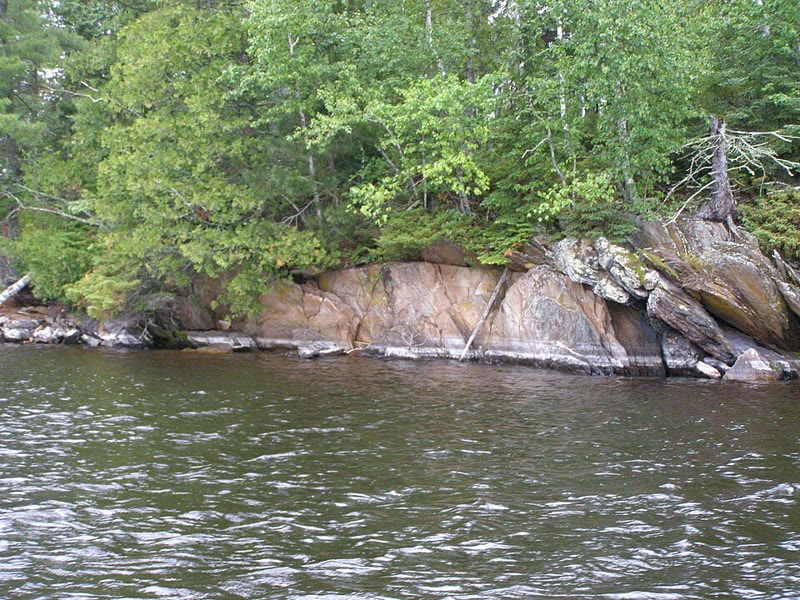
\includegraphics[height=5.0cm]{images/book2/g12-light-canadian-shield.jpg}

{\small Gneisen en granieten van 1 tot 3 miljard jaar oud aan een meeroever in
Canada, een deel van de oude kern van Noord-Amerika. Foto Chris Light
(CC~BY-SA~4.0).}
\end{omfigure}
% ledger: photo:g12-canadian-shield

Waarom blijft de \omterm{def:g12:continental-crust:continental-crust}{continentale korst} bestaan, terwijl de oceaanbodem altijd jong is?
De \omterm{def:g11:ocean-ridges:oceanic-lithosphere}{oceanische korst} is dicht: ze zinkt bij \omterm{def:g11:subduction-zones:subduction}{subductiezones} terug in de mantel,
en niets ervan overleeft veel langer dan 200 miljoen jaar. De \omterm{def:g12:continental-crust:continental-crust}{continentale
korst} is te licht om te zinken; ze kan door erosie worden afgesleten, uitgerekt of
verfrommeld, maar ze blijft aan het oppervlak. De gesteenten van een continent zijn een
archief van vier miljard jaar.
% ledger: tulane:no-subduct, tulane:roots, data:b2-seafloor-age

\section{Bergwortels}

Hoe hoger de bergen, hoe dikker de korst eronder.

\begin{definition}[Bergwortel]\label{def:g12:continental-crust:root}
De \emph{wortel}\index{wortel (van een gebergte)} van een gebergteketen is
het deel van haar verdikte korst dat tot in de mantel reikt, onder het
niveau van de \omterm{def:g11:seismic-structure:moho}{Moho} onder de omringende laaglanden.
\end{definition}
% ledger: tulane:roots

Het model van Airy voorspelt de \omterm{def:g12:continental-crust:root}{wortel}: een keten die $h$ boven haar
omgeving uitsteekt, heeft een \omterm{def:g12:continental-crust:root}{wortel} $r = h\,\rho_c/(\rho_m - \rho_c)$, ongeveer vijf keer
haar hoogte met $\rho_c = \qty{2830}{kg/m^3}$ en $\rho_m =
\qty{3380}{kg/m^3}$ (\cref{prop:g11:lithosphere-asthenosphere:airy}). Twee
soorten metingen zien de \omterm{def:g12:continental-crust:root}{wortels}. Seismisch onderzoek vindt de \omterm{def:g11:seismic-structure:moho}{Moho} dieper
onder ketens: 50 tot \qty{70}{km} onder veel gebergtegordels, ongeveer
\qty{70}{km} onder delen van Tibet. De zwaartekracht is boven gebergteketens zwakker dan
hun zichtbare massa zou doen verwachten: de lichte \omterm{def:g12:continental-crust:root}{wortel}, die de plaats inneemt van
dichtere mantel, vormt een massatekort op diepte, en de gemeten
zwaartekrachtsanomalieën volgen de topografie en de dikte van de korst die de
seismologie vindt. De continenten drijven, en hun bergen drijven het hoogst.
% ledger: tulane:roots, karplus:tibet-moho, cm95:crust, data:prem

\section{Oefeningen}

\begin{exercise}[$\star$]\label{exo:g12:continental-crust:1}
Neem over en vul aan voor de continentale en de \omterm{def:g11:ocean-ridges:oceanic-lithosphere}{oceanische korst}: dikte;
belangrijkste gesteenten; silicagehalte; dichtheid; grootste ouderdom.
\end{exercise}

\begin{exercise}[$\star$]\label{exo:g12:continental-crust:2}
De hele \omterm{def:g12:continental-crust:continental-crust}{continentale korst} bevat \qty{60.6}{\percent} silica, haar bovenste
deel \qty{66.6}{\percent}. Is elk, volgens de silicaklassen van stollingsgesteenten,
\omterm{def:g11:igneous-rocks:felsic-mafic}{mafisch}, \omterm{def:g11:igneous-rocks:felsic-mafic}{intermediair} of \omterm{def:g11:igneous-rocks:felsic-mafic}{felsisch}? Noem een \omterm{def:g11:igneous-rocks:volcanic-plutonic}{plutonisch gesteente} met dezelfde
samenstelling.
\end{exercise}

\begin{exercise}[$\star$]\label{exo:g12:continental-crust:3}
Waarom kan de \omterm{def:g11:ocean-ridges:oceanic-lithosphere}{oceanische korst} bij een \omterm{def:g11:subduction-zones:subduction}{subductiezone} in de mantel zinken, en
de \omterm{def:g12:continental-crust:continental-crust}{continentale korst} niet? Antwoord met dichtheden.
\end{exercise}

\begin{exercise}[$\star$]\label{exo:g12:continental-crust:4}
(1) Wat is een \omterm{def:g12:continental-crust:craton}{kraton}? (2) Hoe oud zijn de gesteenten van een \omterm{def:g12:continental-crust:craton}{kraton} minstens?
(3) Welke soorten gesteenten vormen het?
\end{exercise}

\begin{exercise}[$\star$]\label{exo:g12:continental-crust:5}
De oudste oceaanbodem is ongeveer 190 miljoen jaar oud, de gneis van Acasta
4.03 miljard jaar. Hoeveel keer ouder is de gneis? Waarom is er geen
oceaanbodem die even oud is?
\end{exercise}

\begin{exercise}[$\star\star$]\label{exo:g12:continental-crust:6}
De \omterm{def:g12:continental-crust:continental-crust}{continentale korst} beslaat \num{210.4}~miljoen~\unit{km^2}, waarvan
\qty{30.6}{\percent} onder zee ligt. (1) Welke oppervlakte \omterm{def:g12:continental-crust:continental-crust}{continentale korst}
ligt onder zee? (2) Welke oppervlakte steekt erboven uit? (3) Het aardoppervlak is
$4\pi R^2$ met $R = \qty{6371}{km}$. Welk aandeel van het oppervlak beslaat de
\omterm{def:g12:continental-crust:continental-crust}{continentale korst}?
\end{exercise}

\begin{exercise}[$\star\star$]\label{exo:g12:continental-crust:7}
Bereken de massa van een kolom korst met een doorsnede van \qty{1}{m^2},
van het oppervlak tot de \omterm{def:g11:seismic-structure:moho}{Moho}: (1) door \qty{41.1}{km} \omterm{def:g12:continental-crust:continental-crust}{continentale
korst} met \qty{2830}{kg/m^3}; (2) door \qty{7.1}{km} \omterm{def:g11:ocean-ridges:oceanic-lithosphere}{oceanische korst} met
\qty{3000}{kg/m^3}. (3) Hoeveel keer zwaarder is de eerste?
\end{exercise}

\begin{exercise}[$\star\star$]\label{exo:g12:continental-crust:8}
Een keten staat \qty{2.5}{km} boven laaglanden waarvan de korst \qty{35}{km}
dik is. Bereken met $\rho_c = \qty{2830}{kg/m^3}$ en $\rho_m =
\qty{3380}{kg/m^3}$ haar \omterm{def:g12:continental-crust:root}{wortel} en de dikte van haar korst. Ligt
het resultaat in het bereik dat onder gebergtegordels is gemeten?
\end{exercise}

\begin{exercise}[$\star\star$]\label{exo:g12:continental-crust:9}
Uit het histogram van de ouderdommen van de oceaanbodem: (1) welk aandeel van de oceaanbodem is
jonger dan 30 miljoen jaar? (2) Welke band van 10 miljoen jaar bevat de
meeste bodem? (3) Waarom daalt het aandeel naar hoge ouderdommen toe?
\end{exercise}

\begin{exercise}[$\star\star$]\label{exo:g12:continental-crust:10}
In kaart gebracht met haar ondergelopen delen heeft de \omterm{def:g12:continental-crust:continental-crust}{continentale korst} een gemiddelde hoogte van
ongeveer \qty{120}{m}. Stel dat haar ondergelopen delen, \qty{30.6}{\percent} van haar
oppervlakte, gemiddeld \qty{100}{m} onder zeeniveau liggen. Wat is de gemiddelde hoogte van
haar opgedoken deel? Waarom geven oudere schattingen, die alleen het land telden, een
veel grotere gemiddelde hoogte?
\end{exercise}

\begin{exercise}[$\star\star$]\label{exo:g12:continental-crust:11}
Een boorgat op een eiland ver in een oceaan bereikt, onder een paar honderd
meter lava's, een \omterm{def:g11:ocean-ridges:gabbro}{gabbro}; seismische profielen leggen de \omterm{def:g11:seismic-structure:moho}{Moho} op \qty{8}{km} diepte.
Een ander boorgat, onder een brede, vlakke vlakte, bereikt gneis op \qty{2}{km},
en de \omterm{def:g11:seismic-structure:moho}{Moho} ligt op \qty{38}{km} diepte. Gebruik de methode om te bepalen welke korst
onder elk ligt.
\end{exercise}

\begin{exercise}[$\star\star\star$]\label{exo:g12:continental-crust:12}
Hoe goed is de benadering van de propositie? (1) Bereken het exacte
volume van een schil met dikte \qty{41.1}{km} aan het oppervlak van een bol met
straal \qty{6371}{km}, $\tfrac{4}{3}\pi\bigl(R^3 - (R - H)^3\bigr)$, en het
benaderde volume, $4\pi R^2 H$. (2) Wat is het relatieve verschil? Vergelijk
het met $H/R$.
\end{exercise}

\begin{exercise}[$\star\star\star$]\label{exo:g12:continental-crust:13}
Stel dat het bovenste derde van de \omterm{def:g12:continental-crust:continental-crust}{continentale korst}, naar massa,
\qty{66.6}{\percent} silica bevat, en de hele korst \qty{60.6}{\percent}. (1)
Wat is het silicagehalte van de onderste twee derde? (2) Met welke klasse van
stollingsgesteenten komt het overeen? (3) Wat zegt dat over de diepe
\omterm{def:g12:continental-crust:continental-crust}{continentale korst}?
\end{exercise}

\begin{exercise}[$\star\star\star$]\label{exo:g12:continental-crust:14}
Stel dat er bij de ruggen ongeveer \qty{3}{km^2} nieuwe \omterm{def:g11:ocean-ridges:oceanic-lithosphere}{oceanische korst} per
jaar ontstaat, en dat de oceaanbodem ongeveer \num{300}~miljoen~\unit{km^2} beslaat. (1)
Hoe lang zouden de ruggen erover doen om een oppervlakte gelijk aan de hele
oceaanbodem te maken? (2) Vergelijk met de ouderdommen van de oceaanbodem. (3) Wat moet er gebeuren met
de oude bodem?
\end{exercise}

\begin{exercise}[$\star\star\star$]\label{exo:g12:continental-crust:15}
Stel dat alle \omterm{def:g12:continental-crust:continental-crust}{continentale korst}, \qty{8.6e9}{km^3}, sinds 4.0 miljard jaar geleden
in een constant tempo was ontstaan. (1) Bereken het tempo in kubieke kilometer per
jaar. (2) De zirkoonkorrels van de Jack Hills tonen dat er al wat korst bestond
4.4 miljard jaar geleden. Past een constant tempo bij een wereld waarin het grootste deel van de
korst vroeg is ontstaan, of laat? Wat kunnen de oudste gesteenten vertellen, en
wat niet, gezien dat oude korst kan worden geërodeerd of gerecycled?
\end{exercise}

\section{Probleem: hoe zwaar is de continentale korst?}

\begin{problem}[{Weekendprobleem --- de massa van de continenten}]
\label{pb:g12:continental-crust:1}
% ledger: cogley84:continents, cm95:crust, earth:mass, earth:Rmean, earth:density, white92:crust
% values: 4 pi R^2 = 5.1006e8 km2; V = 210.4e6 x 41.1 = 8.647e9 km3; m = 2.447e22 kg; m/M = 0.410 %
De \omterm{def:g12:continental-crust:continental-crust}{continentale korst} beslaat \num{210.4}~miljoen~\unit{km^2} (ondergelopen delen
inbegrepen). Seismisch onderzoek geeft haar een gemiddelde dikte van \qty{41.1}{km} en
een gemiddelde dichtheid van \qty{2830}{kg/m^3}. De Aarde heeft een gemiddelde straal van
\qty{6371}{km}, een massa van \qty{5.9722e24}{kg} en een gemiddelde dichtheid van
\qty{5513}{kg/m^3}.

\medskip
\noindent\textbf{Deel I --- De oppervlakte.}
\begin{enumerate}
  \item Bereken de oppervlakte van het aardoppervlak, $4\pi R^2$, in
        \unit{km^2}.
  \item Welk aandeel ervan beslaat de \omterm{def:g12:continental-crust:continental-crust}{continentale korst}?
  \item \qty{30.6}{\percent} van de \omterm{def:g12:continental-crust:continental-crust}{continentale korst} ligt onder zee.
        Welke oppervlakte is dat?
  \item Welke oppervlakte van het aardoppervlak blijft over voor de \omterm{def:g11:ocean-ridges:oceanic-lithosphere}{oceanische korst},
        als je aanneemt dat de rest helemaal oceanisch is?
  \item Waarom is de \omterm{def:g12:continental-crust:continental-crust}{continentale korst} groter dan het land?
\end{enumerate}

\medskip
\noindent\textbf{Deel II --- Dikte en volume.}
\begin{enumerate}[resume]
  \item Waarom mag het volume worden berekend als oppervlakte maal dikte, hoewel de
        korst op een bol ligt?
  \item Bereken het volume van de \omterm{def:g12:continental-crust:continental-crust}{continentale korst} in \unit{km^3}.
  \item Reken het om naar \unit{m^3}.
  \item Een andere schatting van de gemiddelde dikte is \qty{36}{km}. Welk
        volume geeft die?
  \item Hoeveel procent verschillen de twee volumes?
\end{enumerate}

\medskip
\noindent\textbf{Deel III --- Dichtheid en massa.}
\begin{enumerate}[resume]
  \item Bereken de massa van de \omterm{def:g12:continental-crust:continental-crust}{continentale korst} met \qty{41.1}{km}.
  \item Bereken de massa van een kolom van \qty{1}{m^2} door de \omterm{def:g12:continental-crust:continental-crust}{continentale
        korst}.
  \item Bereken de massa van de \omterm{def:g11:ocean-ridges:oceanic-lithosphere}{oceanische korst}: oppervlakte uit vraag~4,
        dikte \qty{7.1}{km}, dichtheid \qty{3000}{kg/m^3}.
  \item Welke is zwaarder, en hoeveel keer? Waarom, hoewel ze minder
        oppervlakte beslaat?
  \item Waarom is de \omterm{def:g12:continental-crust:continental-crust}{continentale korst} minder dicht dan de \omterm{def:g11:ocean-ridges:oceanic-lithosphere}{oceanische korst}?
\end{enumerate}

\medskip
\noindent\textbf{Deel IV --- Vergeleken met de Aarde.}
\begin{enumerate}[resume]
  \item Deel de massa van vraag~11 door de massa van de Aarde.
  \item Controleer het resultaat met de propositie over dunne lagen.
  \item Welk aandeel van de massa van de Aarde is de \omterm{def:g11:ocean-ridges:oceanic-lithosphere}{oceanische korst}?
  \item De \omterm{def:g12:continental-crust:continental-crust}{continentale korst} bevat de enige gesteenten die ouder zijn dan ongeveer 200
        miljoen jaar. Welk aandeel van de massa van de Aarde draagt het archief van
        bijna haar hele geschiedenis?
  \item Besluit: welk aandeel van de massa van de Aarde is de \omterm{def:g12:continental-crust:continental-crust}{continentale korst}?
\end{enumerate}
\end{problem}
